%*******************************************************************************
%****************************** Second Chapter *********************************
%*******************************************************************************

\chapter{The execution semantic of Flink Stream Processing}

\ifpdf
    \graphicspath{{Chapter3/Figs/Raster/}{Chapter3/Figs/PDF/}{Chapter3/Figs/}}
\else
    \graphicspath{{Chapter3/Figs/Vector/}{Chapter3/Figs/}}
\fi

\section{Heterogeneity}\label{Heterogeneity}
Since the first commercial project of Complex Event Processing launched by Bell Labs in 1998 with its "Sunrise Project", we have seen the fast growing of many stream processing frameworks. However, there is a huge degree of heterogeneity across these frameworks in various forms \citep{Dindar:2013}: 

\begin{enumerate}

	\item \textbf{Syntax}: Although the ISO/IEC 9075 is published to standardize the complete syntax and operations in SQL language as a whole, there is no standard language for stream processing. Different stream processing engines use different syntax to depict the same semantic meaning. For example, every 5 seconds, a window captures all event last 10 seconds. 
	\begin{verbatim}
	CQL: 	[RANGE 10 seconds SLIDE 5 second ] 
	Flink: 	[SIZE 10 sec EVERY 5 sec]
	\end{verbatim}
	
	\item \textbf{Capability heterogeneity}:
	Those engines also provide different set of query types and operations based on which functions they are capable of. For examples, \textit{Streambase} support pattern matching on stream, whereas STREAM does not.
	
	\item \textbf{Execution Model}: Below the language level, hidden from application layers, each stream processing engine has its own underlying execution model. With the same data stream but different model produce different output which varies based on the differences on tuple ordering,  window construction, evaluation and so on. We are going to focus on the differences between several existing execution models below.
	
	
\end{enumerate}
 
We have learned that there are at least three different execution models:
\begin{itemize}
	\item \textbf{Time-driven} execution model, followed by CQL, Oracle CEP. In the model, each tuple have a timestamp. Timestamp induces the total order of tuples on stream, but not a strict total order. Or more specifically, there is no ordering between tuples with identical timestamps. These tuples are considered as simultaneous tuples. It is problematic when we select a window of last 10 tuples but more than 10 simultaneous tuples arrived at a given time instant. In this case, there is no different between those tuples, the system will select only 10 out of all in a non-deterministic way.
	
Assuming that we has stream $\mathbb{S}$ (regardless of system timestamps): 
	\begin{equation}
			\mathbb{S}(value, t_{app}) = s_1(1,1),\,\,s_2(10,2),\,s_3(20,2),\, s_4(100,3)
	\end{equation}
	

	
Consider a query which continuously recall the last arrival tuple i.e., we select tuple-based window with size of 1 tuple. In the time-based execution model,  the state of a window changes as timestamp progress. Window gets re-evaluated only when timestamp change. At $t=1$ or $t=3$, there is only 1 tuple arrived, new 1-tuple-size window will open , pick the tuple then close. Thus the stream derives window $W_1: \{s_1(1,1)\}$ and $W_3: \{s_4(100,3)\}$. On the other hand, at $t=2$, there are 2 new tuple arrivals simultaneously. New window $W_2$ opens and accepts 1 tuple only. Since these 2 tuples arrive simultaneously, they will have the same timestamp and thus no any temporal differences between them. System simply picks one of them randomly for window $W_2$. In short, window $W_2$ contains one of following options: $s_2(10,2)$ or $s_3(20,2)$. The derived stream will be one of the streams:
\begin{equation}
W_1\{s_1\},\, W_2\{s_2\},\, W_3\{s_4\}\, \textit{or}\, W_1\{s_1\},\, W_2\{s_3\},\, W_3\{s_4\}
\end{equation}

\begin{figure}[htbp!] 
\centering    
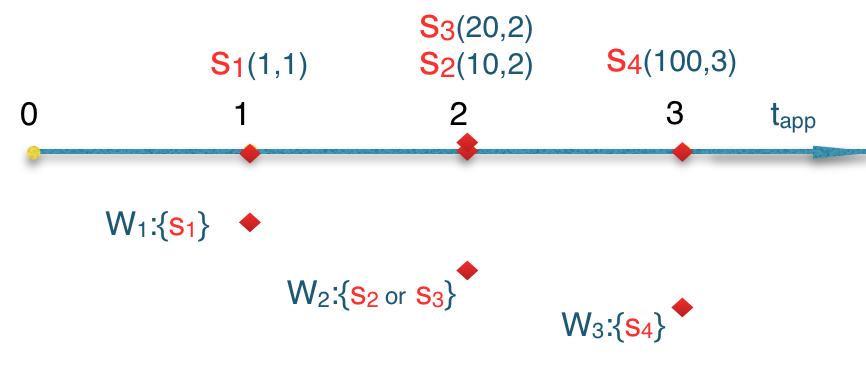
\includegraphics[width=0.7\textwidth]{time-driven}
\caption{Time-driven Execution model. Window size of 1 tuple}
\label{fig:time-driven}
\end{figure}
	
	\item \textbf{Tuple-driven} execution model, followed by StreamBase, Apache Flink. In this model, tuples may have an application timestamp attribute on its schema. Some of application timestamp values might be identical but tuples themselves are completely distinguished in stream. There exists a strict total order in stream based on their arrival order. 
	
	There are several ways to represent tuple order in stream. StreamBase system assigns an incremental internal rank to tuples to arriving tuples. It ensures that the tuple with lower rank with be processed before tuples with higher ranks. In Apache Flink, we implicitly use system timestamp   $t_{sys}$ at which system receives the tuple. Executing this \textit{tuple-at-a-time} model, logically Flink places new arrived tuple to a queue and process it one by one. Therefor, there is at most one tuple  considered arriving at a give time.  Since tuples with attached system timestamps are strictly totally ordered, it is perfectly suitable for Flink's execution model. Several other works propose to use tuple Id \citep{Dindar:2013} or a physical identifier\citep{Petit:2010} instead. 	
	
	In tuple-driven execution model, each tuple arrival cause a system to react, instead of each application timestamp progress. 
	
	Extending previous examples, every tuple is entitled to a system timestamp. As we mentioned in previous chapter, application and system timestamp are not necessarily synchronized.
	\begin{equation}
			\mathbb{S}(value, t_{app}, t_{sys}) = s_1(1,1,28),\,\,s_2(10,2,37),\,s_3(20,2,40),\, s_4(100,3,46)
	\end{equation}
	
	Tuple $s_2$ and $s_3$ has the same application timestamp $t_{app} = 2$ but system will open a separate 1-tuple-size window for each of them upon their arrivals. Therefore, since $s_2$ arrived before $s_3$, the derived stream will be exact as (Figure \ref{fig:tuple-driven})
	\begin{equation}
W_1\{s_1\},\, W_2\{s_2\},\, W_3\{s_3\}\,W_4\{s_4\}
\end{equation}
	
	\begin{figure}[htbp!] 
\centering    
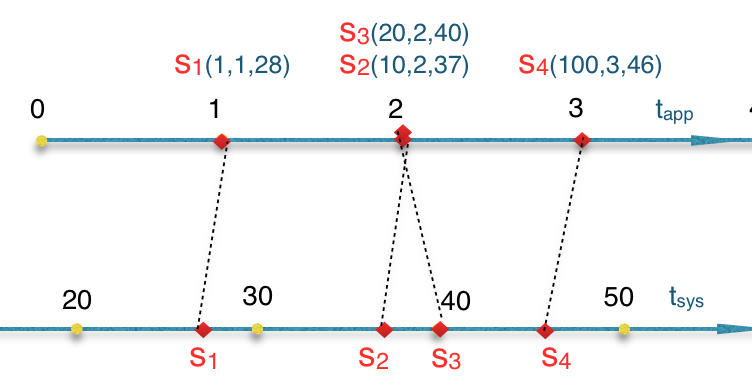
\includegraphics[width=0.6\textwidth]{tuple-driven}
\caption{Tuple-driven Execution model}
\label{fig:tuple-driven}
\end{figure}
	
	\item \textbf{Batch-driven} execution model, followed by Coral8, mentioned in SECRET\citep{Botan:2010} descriptive model 
	
	
In this model, every tuple is assigned an batch-id. Tuples which belong to a batch must have the same timestamp, but two separate tuples with the identical timestamp may belong to two different batches. As we can see, batch-driven model is in between of tuple-driven and time-driven model (Figure~\ref{fig:executionModel}). Assuming that at a given application timestamp $t_{app} = 2$, the system receives 5 tuples $\{s_1,\,s_2,\,s_3,\,s_4,\,s_5\>\}$,  but they arrive at different $t_{sys}$ respectively. Time-driven model treats them as simultaneous tuples with no difference. Tuple-driven considers them as 5 concrete tuples in strict order. And batch-driven model may divide them into 2 batches $\{s_1,\,s_2,\,s_3\}$, $\{s_4,\,s_5\}$ depending on window specification.



\begin{figure}[htbp!] 
  \centering
  \begin{subfigure}[b]{0.3\textwidth}
    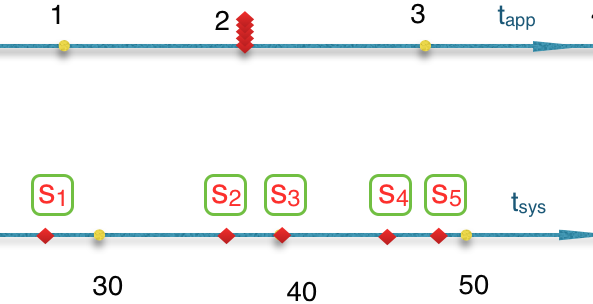
\includegraphics[width=\textwidth]{executionModel_a}
    \caption{Tuple-driven}
    \label{fig:TomJerry}   
  \end{subfigure}             
  \begin{subfigure}[b]{0.3\textwidth}
    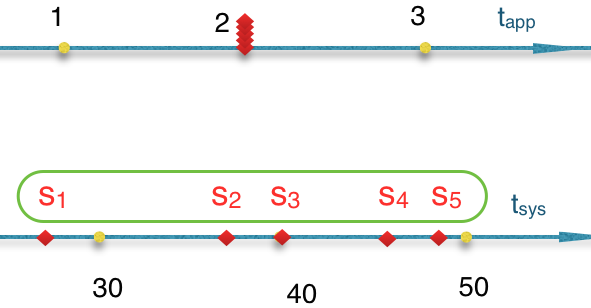
\includegraphics[width=\textwidth]{executionModel_b}
    \caption{Time-driven}
    \label{fig:WallE}
  \end{subfigure}             
  \begin{subfigure}[b]{0.3\textwidth}
    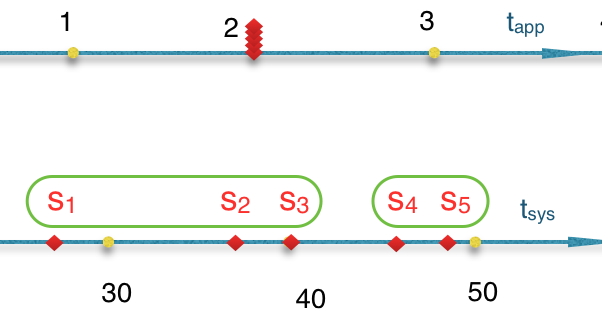
\includegraphics[width=\textwidth]{executionModel_c}
    \caption{Batch-driven}
    \label{fig:Minnion}
  \end{subfigure}
  \caption{Execution models}
  \label{fig:executionModel}
\end{figure}

\end{itemize}
We extends the examples in \citep{Dindar:2013} with Flink implementation in order to demonstrate that system with different execution model may produce different output , even with the same input and query. 
\begin{enumerate}

\item \textbf{Example 1:} \textit{differences in window constructions}.

Given \textit{Instream} stream with schema $S(time, value)$. Consider a query which continuously computes the average value of tuples in a time-based tumbling window of size 3.
\begin{align*}
Instream(time,value) &= \{(10,10),(11,20),(12,30),(13,40),(14,50),\\
&\qquad (15,60),(16,70),...\} \\
Oracle\, CEP\, (avg)		&= \{(20), (50),...\} \\
Flink\, (avg)			&= \{(15), (40),...\} \\
\end{align*}

Obviously, Oracle CEP constructs the first window with first 3 tuples whereas Flink picks first 2 tuples only. The second window , they both take next 3 tuples. We implement the test on Flink with default configuration, however we are able to customize the upper bound of the first window ($startTime = 12$)so that it produces the same result as Oracle CEP.


\item \textbf{Example 2:} \textit{differences in window evaluations}.

Consider a query which continuously computer the average value of tuples over last 5 second once every 1 second (time-based window of size 5s that slides by 1s)

\begin{align*}
Instream(time,value) 	&= \{s_1(30,10),\,s_2(31,20),\,s_3(36,30),...\} \\
Oracle\, CEP\, (avg)		&= \{(10), (15),(20),...\} \\
Flink\, (avg)			&= \{(10), (15), (15), (15), (15), (20),...\}\\
Coral8\, (avg)			&= \{(10), (15),(20),...\}			
\end{align*}

Flink produced a different result than Oracle and Coral8.
In Oracle and Coral8, a new window is emitted for invoking the average operator only when the window content's change; whereas in Flink, it emits a new window every second as the sliding progress , even if the content does not change. The state of window is depicted on Figure ~\ref{fig:winEvaluation}
\begin{figure}[htbp!] 
\centering    
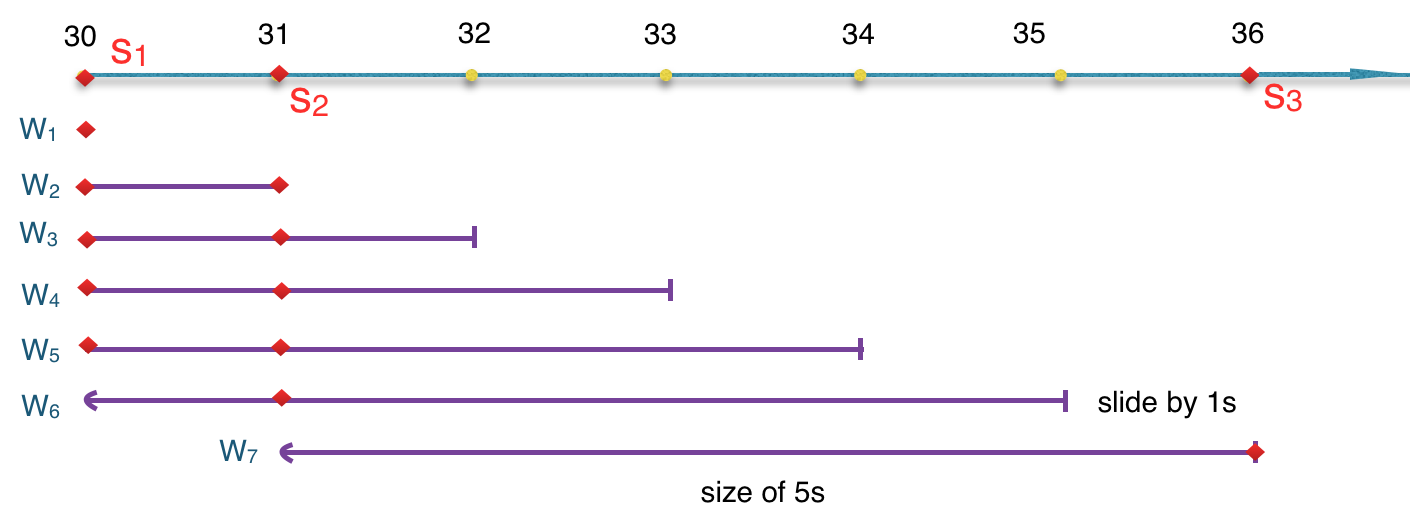
\includegraphics[width=0.8\textwidth]{winEvaluation}
\caption{Window Evaluation}
\label{fig:winEvaluation}
\end{figure}

Remember that window closes at upper boundary and opens at lower boundary so that in window $W_6$ cover from $t=35$ to right after $t=30$ will exclude tuple $s_2(30,10)$. Similarly, $W_7$ excludes tuple $s_3(31,20)$

\item \textbf{Example 3:} \textit{differences in processing granularity}.

Consider a query which computes the average value of tuples over a tuple-based tumbling window of size 1 tuple.
\begin{align*}
Instream(time,value) 	&= \{(10,10),(10,20),\\
						&\quad (11,30),\\
						&\quad (12,40),(12,50),(12,60),(12,70),\\
						&\quad (13,80),...\} \\
Oracle\, CEP\, (avg)		&= \{(20), (30),(70),(80)...\} \\
Flink\, (avg)			&= \{(10), (20), (30), (40), (50), (60),(70),(80)...\}\\
Coral8\, (avg)			&= \{(10), (20), (30), (40), (50), (60),(70),(80)...\}
\end{align*}

Oracle CEP implements time-based execution model so that it reacts to each application timestamp. If there are multiple simultaneously tuple arrive, it will pick one of them non-deterministically to construct the window , since window size is 1. In other hand, Flink and Coral8 react to every tuple arrival so that they emit new 1-tuple-size tumbling window for every tuple.

\end{enumerate}


tuple: each tuple arrival cause a system to react
time: the progress of tapp cause a system to react
batch:  where either a new batch arrival or the progress of tapp cause a system to react


\textbf{TODO} http://blog.mikiobraun.de/2014/01/apache-spark.html


\section{Policy-based Window Semantics in Flink}


Flink constructs windows based on parameters in specification. Currently Flink does not support Predicate Window so that two of most critical parameters are to notify when system should trigger new windows (indicating the lower bound of window) and when system must end the window (indicating the upper bound of window) and emit it to window stream. For that purpose, Flink implements a mechanism called \textit{"Policy-based windowing"}. It is a highly flexible way to specify stream descretization. It has two independent policies corresponding to open and re-evaluate a window: Trigger and Eviction Policy.
To demonstrate the concepts of two policies, let's consider the scenario with \textit{StockTick} stream: check every 10 minutes the total transaction volume of all transaction last 30 minutes. In other words, in every 10 minutes create a new window to cover all the transactions in last 30 minutes. The syntax in Fink:

\begin{verbatim}
StockTick.window(Time.of(30, MINUTES))
		 .every(Time.of(10, MINUTES)).sum(Quantity)
\end{verbatim}

\begin{enumerate}

\item \textbf{Eviction Policy}: define the length of a window. The length is passed in to \textit{window(...)} function. It could be the time interval, number of tuples and delta function with threshold (in case of delta window).
We formalize the concept of window due to its size

\begin{defi}
A time-based window $W_{t} = (l,u,\omega_t)$ over a stream $S$ is a finite subset of  $\mathbb{S}$ containing all data elements $s \in \mathbb{S}$ where $l , u, \omega_t \in \mathbb{T}$ and $l < s.t \leq u$. The length of window in time unit is $\omega_t = u-l$
\end{defi}
Notice that in a time-based window, $s.t$ can be tuple's application or system timestamp depending on query. Again, there are maybe many simultaneous tuples with an identical $t_{app}$. However, there is at least one arriving tuple at a given $t_{sys}$. The second point is that $W_t$ open at $t = l$, it does not include tuple at this time instant.

\begin{defi}
A count-based window $W_{c} = (l,u,\omega_c)$ over a stream $S$ is also a finite subset of  $\mathbb{S}$ containing all data elements $s \in \mathbb{S}$ where $l,u \in \mathbb{T}$, $\omega_c \in \mathbb{N}$ and $l \leq s.t_{sys} \leq u$. The length of window $\omega_c$ is the number of tuples in interval time $[l, u]$, i.e., $\omega_c = | {s \in \mathbb{S}(t_{sys}): l \leq s.t_{sys} \leq u}|$
\end{defi}
The count-based window $W_{c}$ is independent from application timestamp $t_{app}$. It is only related to system timstamp $t_{sys}$ which indicates tuple's order in stream. 


\item \textbf{Trigger Policy}: In general, it defines window slide or the distance between 2 consecutive windows. On above example , trigger policy states that from beginning, system must trigger a new window every 10 minutes. No other window would be triggered in between.

Supposed that we have 2 consecutive windows $W_1 = (l_1, u_1, \_)$ and $W_2 = (l_2, u_2, \_)$  where $l_1 < l_2$. There is no window $W' = (l_3, u_3, \_)$ such that $l_1< l_3 < l_2$.
\begin{defi}
The distance or slide between 2 windows $W_1$ and $W_2$ is the distance between two of their upper-bound tuple as
\begin{itemize}


\item  A time-based slide $\beta_{t} = u_2 - u_1$.  
\item A count-based slide $\beta_{c} = |{s \in \mathbb{S}(t_{sys}): u_1 < s.t_{sys} \leq u_2}| $ 

\end{itemize}

\end{defi}

\end{enumerate}

There is a correlation between window size and slide size  conforming to the movement type of windows.
\begin{itemize}
\item Sliding window: $\omega > \beta$ or $n > e$
\item Tumbling window: $\omega = \beta$ or $n = e$
\item Jumping window: $\omega < \beta$ or $n < e$
\end{itemize}

However, Flink allows to mix between time-based trigger policy with count-based eviction policy and vice versa. For example,
calculate sum of quantities of last 100 transactions every 1 hour.
\begin{verbatim}
StockTick.window(Count.of(100))
		 .every(Time.of(1, HOURS)).sum(Quantity)
\end{verbatim}

\section{The execution models in Flink}
We present here the execution models of Flink Stream Processing engine. Tick model specifies how the engine reacts to new tuple arrival while Window Construction show the way Flink constructs and emits a complete window based on window specifications. There are pretty many reviews on window construction (\textbf{\\TODO}: which?) ... However, none of them give a full description in the case that we mix up time-based and count-based specification for window size and slide.  


%\begin{verbatim}
%
%		boolean isTriggered = false;
%
%		if (triggerPolicy.notifyTrigger(input)) {
%			emitWindow();
%			isTriggered = true;
%		}
%
%		evict(input, isTriggered);
%
%		collector.collect(windowEvent.setElement(input));
%		bufferSize++;
%
%\end{verbatim}

Window Buffer \textit{wb} is a linking list contain tuples with composite type $IN$



%\begin{equation}
%	t = 
%	\begin{cases}
%		t_{sys} \qquad if\,t_{app} = None\\
%		   \\
%		t_{app} \qquad\qquad\qquad otherwise
%	\end{cases}
%\end{equation}

$size_{t}(wb) = wb.last.t - wb.first.t$

$size_c(wb) = wb.length()$


\begin{algorithm}
\caption{Process new arrived tuple}
\label{algorithm:processNewTuple}
The first step, before processing a new arrived tuple, check if a current window buffer should be emitted. If yes, copy the current window buffer to a window object and put to Windowed Stream. The second step, calculating which tuples should be evicted if the current window buffer appends new arrived tuple. There are two separate case for time-based and tuple-based window. The third step, evicting those tuples and appending new arrived tuple.


\algrenewcommand\algorithmicfunction{\textbf{class}}
\algrenewcommand\algorithmicprocedure{\textbf{method}}
  \begin{algorithmic}[1]
  	\Require {$wb$: the current window buffer}
  	
  			{$\omega_t$: size of window in time interval }
  			
  			{$\omega_c$: size of window in tuple count }
    %\Function{Mapper}{}
    \Procedure{processNewTuple}{$\textrm{newTuple }: IN$}
    
    \If{$\textsc{notifyTrigger}(newTuple) \textrm{ \& } size_c(wb) > 0$} \Comment{ trigger new window}
    		\State $\textrm{window} \gets \textrm{wb}$
    		\State $\textsc{Emit}(\textrm{window})$ \Comment {emit to Windowed stream}
    \EndIf
    
    \If{$\textrm{window is time-based}$}
    		\State $ evict_t \gets size_t (\textrm{wb.append(newTuple)}) - \omega_t$
    
    		\If{$evict_t > 0$} \Comment {remove old tuples}
    			\State $ \textrm{lastEvictedTimestamp} \gets wb.first.t + evict_t - 1$
    			\ForAll{element $e$ in window buffer $wb$}
    				\If {$e.t \leq \textrm{lastEvictedTimestamp}$}
    					\State $wb.remove(e)$
    				\EndIf
    			\EndFor
    		\EndIf
    \Else \Comment{window is count-based}
    		\State $evict_c \gets size_c(\textrm{wb.append(newTuple)}) - \omega_c$
    		\If{$evict_c > 0$} \Comment {remove old tuples}
    			\For {$i \gets 1, evict_c$}
    				\State $wb.removeFirst()$
    			\EndFor
    		\EndIf
    \EndIf
    
   	\State $wb \gets wb.append(newTuple)$ \Comment {add new tuple to current window buffer}
    
    
    \EndProcedure
    %\EndFunction
  \end{algorithmic}
  




\end{algorithm}


\begin{algorithm}
\caption{Whether system should trigger a new window }
\label{algorithm:notifyTrigger}
When a new tuple has arrive, system check whether the current window buffer reached the point where distance of 2 windows is equal to slide size or not. The new tuple is not really appended to buffer, use it for qualifying purpose only.

\algrenewcommand\algorithmicprocedure{\textbf{method}}
\begin{algorithmic}[1]
  	\Require {$\beta_c$: count-based slide size}
  	
  			{$\beta_t$: time-based slide size }

  			{$lastUpperBound$: timestamp of upper boundaries of previous window}
    %\Function{Mapper}{}
    \Procedure{notifyTrigger}{$\textrm{newTuple }: IN$}
    
   
    
    \If{$\textrm{slide is time-based}$}
    		\If{$(\textrm{newTuple.t} - lastUpperBound) > \beta_t$}
    			\State $\textrm{lastUpperBound} \gets \textrm{lastUpperBound} + \beta_t$
    			\State $\textrm{return true}$
    		\Else
    			\State$\textrm{return false}$
    		\EndIf
    
    \Else \Comment{window is count-based}
    		\If{$\textrm{counter} \geqslant \beta_c $}
    			\State $\textrm{counter} \gets 1$
    			\State $\textrm{return true}$
    		\Else
    			\State $\textrm{counter} \gets \textrm{counter} + 1$
    			\State $\textrm{return false}$
    		\EndIf
    	\EndIf
    
    
    \EndProcedure
    %\EndFunction
  \end{algorithmic}
\end{algorithm}


\subsection{Tick Model}
As we mentioned in \ref{Heterogeneity}, there are three common Tick execution models\citep{Dindar:2013} implemented in various systems. STREAM and Oracle CEP implements time-driven model which reacts once to all tuples with an identical application timestamp. Coral 8 with batch-driven model takes action on an atomic batch which may contain multiple tuples with the same batch-id. Flink and StreamBase with tuple-driven model actively trigger actions on every new arrived tuple.

In Flink, tuples are strictly totally ordered based on its system-assigned timestamp. We describe a procedure taken place on a recent arrived tuple in method \textit{processNewTuple}  (of Algorithm\ref{algorithm:processNewTuple}). 
System takes action on new tuples one by one due to its moment of arrival. 
Basically, Flink employs a linked list as a window buffer to temporarily store a queue of arrived tuples. New tuple will be added to window buffer whereas old tuples will be removed from window buffer according to eviction policy.

Whenever a new tuple has arrived, the procedure is as following:
\begin{itemize}
\item \textbf{Step 1:} The system checks whether the stream reached the point where it should emit the current window buffer to windowed stream and trigger a new window. The condition to trigger a new window is represented in method \textit{notifyTrigger} (in algorithm \ref{algorithm:notifyTrigger}). If the condition is satisfied and window buffer is not empty, system will emit the current window buffer to discretized Windowed Stream for later computation.  

In method \textit{notifyTrigger}, system decides to trigger a new window according to trigger policy defined in window specification. 
Supposed that the previous emitted window is $W^1$, the current window buffer is $wb$, and new arrived tuple $s$.
If the distance between $W^1$ and $\textrm{wb} \bigcup \{s\}$ start exceeding slide size $\beta$ (defined in window specification), system confirms the trigger point and reset the slide measurement:
\begin{itemize}
\item If the slide is time-based, set timestamp of new upper boundaries as \textit{lastUpperBound}
\item If the slide is count-based, reset counter to 1

\end{itemize}

Notice that system has not inserted new tuple to window buffer yet, but at last step.

\item \textbf{Step 2: }evict old tuples in window buffer.
Supposed that system adds new tuple to window buffer, system evicts a number of oldest tuples so that size of the buffer does not exceed pre-defined window size $\omega$. This eviction policy is activated whenever a new tuple has arrived to ensure that window buffer size  never exceed $\omega$
\begin{itemize}
	\item if the window is time-based, time interval cover the window is not bigger than $\omega_t$
	\item if the window is tuple-based, number of tuples in the window does not exceed $\omega_c$
\end{itemize}
\item \textbf{Step 3:} officially insert new tuple to window buffer.
\end{itemize}

In short, we figure out some crucial properties of Tick model in Flink
\begin{itemize}
\item Flink implements tuple-driven model reacting to every new arrived tuple.
\item The eviction policy is to keep size of window buffer shrink shrunk to pre-defined window size $\omega$
\item One is able to mix up different type of window and slide size. For instance, tuple-based window slide by time interval.
\end{itemize}



\subsection{Window Constructions}
We are able to define window and slide size based on application timestamp, system timestamp or number of tuple. Therefore, we have 9 ways to construct a basic window with combination of window and slide size.


\subsubsection{Upper boundary}
In time-based slide,  supposed that $u_1$ is  the upper boundary of the first window. 
The upper boundary of the $k$th window is $u_k = u_1 + k.\beta_t$

\begin{figure}[htbp!] 
\centering    
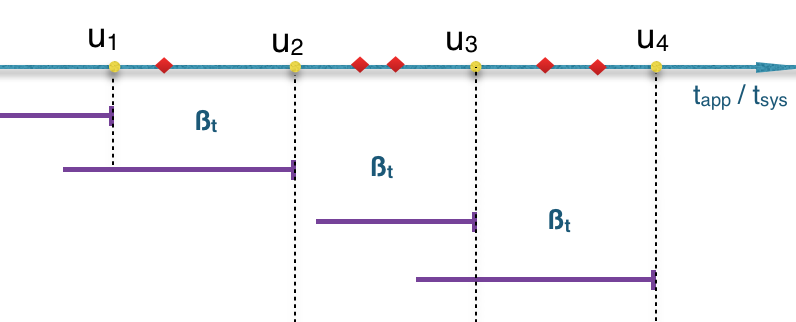
\includegraphics[width=0.5\textwidth]{timebased_slide}
\caption{time-based slide}
\label{fig:timebased_slide}
\end{figure}

In count-based slide, supposed that $u_1$ is the system timestamp of last element of the first window, the last element $s<v,_,t_k>$ of the $k$th window must satisfies $|{s \in \mathbb{S}(t_{sys}): u_1 < s.t_{sys} \leq u_2}| = n.\omega_c$

\begin{figure}[htbp!] 
\centering    
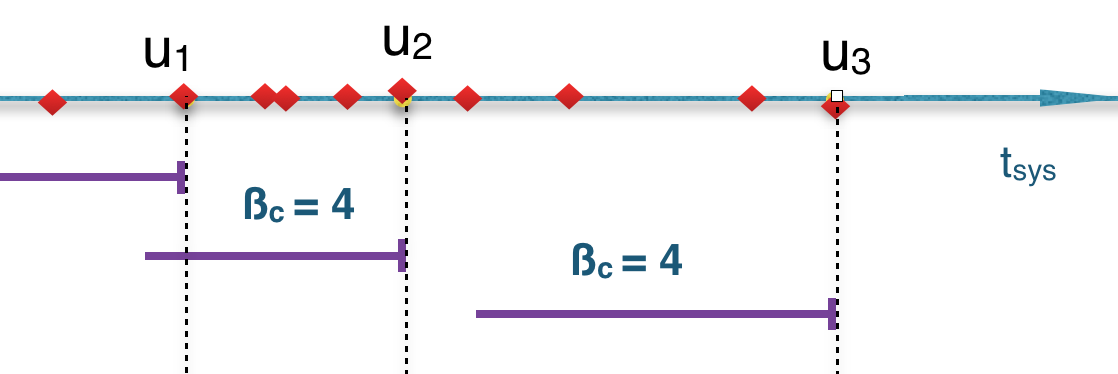
\includegraphics[width=0.5\textwidth]{countbased_slide}
\caption{count-based slide}
\label{fig:countbased_slide}
\end{figure}

\subsubsection{Lower boundary}

In time-based windows, windows are defined in terms of of timestamp. Supposed that we know the upper bound $u_k$ of the $k$ window. The lower bound $l_k = max(0, u_k - \beta_t)$

\begin{figure}[htbp!] 
\centering    
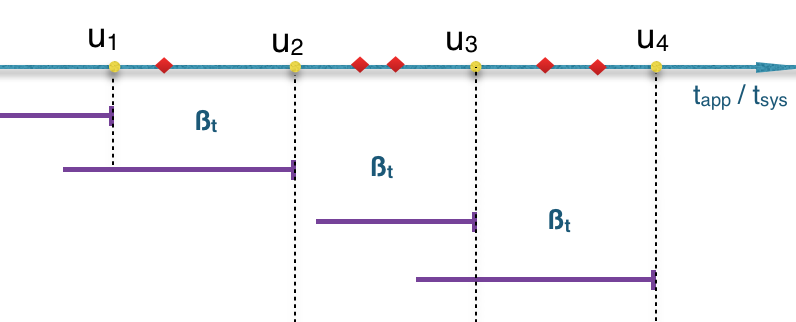
\includegraphics[width=0.5\textwidth]{timebased_slide}
\caption{time-based slide}
\label{fig:timebased_window}
\end{figure}

\begin{itemize}
\item Using application timestamp. The window content is $W = \{s:<v, t_{app},\_> \in \mathbb{S} \wedge max(0, u_k - \omega_{t_{app}}) < t_{app} \leq u_k\}$ where $u_k$ is upper boundary of window in application timestamp unit


\item using system timestamp. The window content is $W = \{s:<v,\_, t_{sys}> \in \mathbb{S} \wedge max (0, u_k - \omega_{t_{sys}}) < t_{sys} \leq u_k\}$ where $u_k$ is upper boundary of window in system timestamp unit
\end{itemize} 


In count-based windows, the scope of window is defined in terms of number of tuples. Thus, given the last tuple $s:<v, \_, u_k>$ of the window. The window content is 
$W=\{s:<v, \_, t_{sys}> \in \mathbb{S} \wedge t_{sys} \leq u_k \wedge  |\{<v,\_,t'_{sys}> \in \mathbb{S} : t_{sys} \leq t'_{sys} \leq u_k\}| \leq \omega_c \}$

\begin{figure}[htbp!] 
\centering    
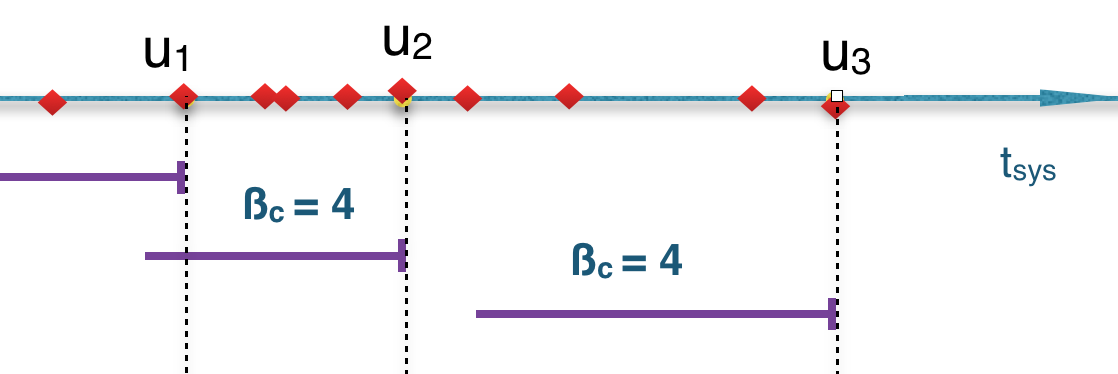
\includegraphics[width=0.5\textwidth]{countbased_slide}
\caption{count-based slide}
\label{fig:countbased_slide}
\end{figure}


\subsubsection*{In case of partitioned group within window}



http://www.sqlstream.com/blog/2015/03/5-reasons-why-spark-streamings-batch-processing-of-data-streams-is-not-stream-processing/